\documentclass[12pt,a4paper]{article}

% ── Packages ──────────────────────────────────────────────────────────────────
\usepackage[T1]{fontenc}
\usepackage[utf8]{inputenc}
\usepackage[margin=2.5cm]{geometry}
\usepackage{graphicx}
\usepackage{booktabs}
\usepackage{tabularx}
\usepackage{array}
\usepackage{multirow}
\usepackage{amsmath}
\usepackage{amssymb}
\usepackage{hyperref}
\usepackage{xcolor}
\usepackage{listings}
\usepackage{caption}
\usepackage{subcaption}
\usepackage{float}
\usepackage{enumitem}
\usepackage{parskip}
\usepackage{lmodern}

% ── Hyperref settings ─────────────────────────────────────────────────────────
\hypersetup{
  colorlinks = true,
  linkcolor  = blue!70!black,
  urlcolor   = blue!70!black,
  citecolor  = red!70!black,
}

% ── Code listing style ────────────────────────────────────────────────────────
\lstset{
  basicstyle  = \ttfamily\small,
  breaklines  = true,
  frame       = single,
  language    = Python,
  numbers     = left,
  numberstyle = \tiny\color{gray},
  keywordstyle= \color{blue},
  commentstyle= \color{green!50!black},
  stringstyle = \color{orange!80!black},
}

% ── Title ─────────────────────────────────────────────────────────────────────
\title{
  \textbf{CENG 467 -- Natural Language Understanding and Generation}\\[0.5em]
  \Large Take-Home Midterm Examination\\[0.5em]
  \normalsize
  \href{https://github.com/nadezhda648/CENG467-Midterm}
       {GitHub Repository (click to open)}
}
\author{
  Student ID: \texttt{290201003}\\
  \texttt{umtarsln0@gmail.com}
}
\date{May 2026}

% ══════════════════════════════════════════════════════════════════════════════
\begin{document}
\maketitle
\tableofcontents
\newpage

% ─────────────────────────────────────────────────────────────────────────────
% Q1
% ─────────────────────────────────────────────────────────────────────────────
% ============================================================
% Q1 – Representation Learning in Text Classification
% ============================================================

\section{Question 1 -- Representation Learning in Text Classification}

\subsection{Dataset Description}

We use the \textbf{IMDb Movie Reviews} dataset~\cite{maas2011imdb}, a widely-used
sentiment classification benchmark. Key properties are summarised in
Table~\ref{tab:q1_dataset}.

\begin{table}[H]
  \centering
  \caption{IMDb Dataset Statistics}
  \label{tab:q1_dataset}
  \begin{tabular}{lrr}
    \toprule
    \textbf{Split} & \textbf{Size} & \textbf{Positive / Negative} \\
    \midrule
    Train & 25{,}000 & 12{,}500 / 12{,}500 \\
    Test  & 25{,}000 & 12{,}500 / 12{,}500 \\
    \midrule
    Total & 50{,}000 & 25{,}000 / 25{,}000 \\
    \bottomrule
  \end{tabular}
\end{table}

The dataset is \textit{perfectly balanced} (50\% positive, 50\% negative), so
random-classifier accuracy equals 50\%.
Mean review length is approximately 233.8 words
(median 174.0),
making IMDb significantly longer than SST-2 and richer in contextual information.

\begin{figure}[H]
  \centering
  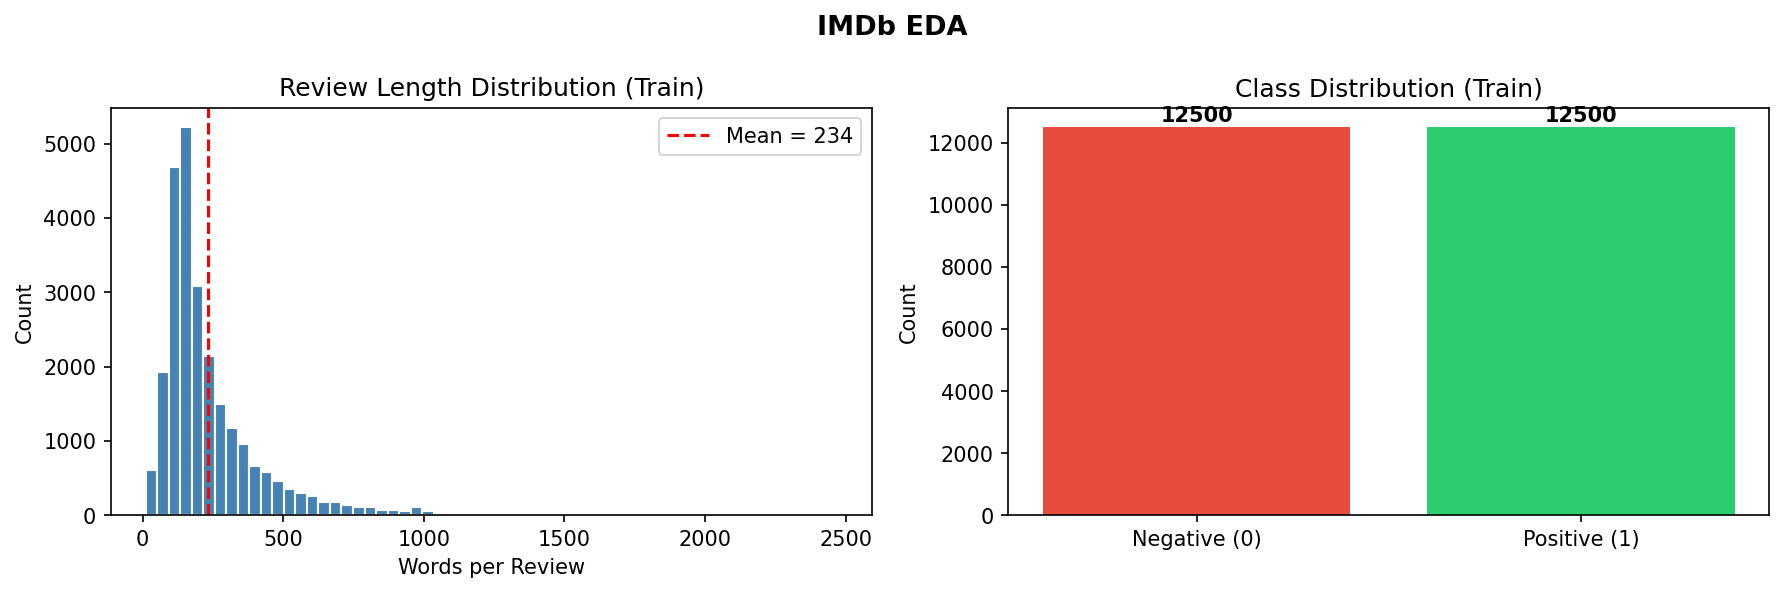
\includegraphics[width=0.85\textwidth]{figures/imdb_eda.png}
  \caption{IMDb dataset EDA: review length distribution (left) and class balance (right).}
  \label{fig:imdb_eda}
\end{figure}

\subsection{Preprocessing Pipeline and Tokenisation Strategies}

We compare two tokenisation strategies.

\paragraph{Strategy 1 – NLTK Word Tokeniser.}
Rule-based, punctuation-aware word splitting (Penn Treebank tokeniser).
Applied to classical and BiLSTM models.
Pipeline steps: (1) HTML tag removal, (2) non-alphanumeric stripping,
(3) lowercasing, (4) optional stopword removal, (5) optional truncation.

\paragraph{Strategy 2 – WordPiece (DistilBERT Tokeniser).}
Subword BPE tokeniser from \texttt{distilbert-base-uncased}, with
\texttt{max\_length=256} and \texttt{[CLS]}/\texttt{[SEP]} special tokens.
WordPiece splits unknown or compound words into sub-units, preserving
morphological information at the cost of ~20--30\% more tokens than Strategy~1.

\subsubsection{Preprocessing Ablation Study}

Table~\ref{tab:q1_ablation} shows the effect of four preprocessing configurations
on TF-IDF + Logistic Regression accuracy.

\begin{table}[H]
  \centering
  \caption{Preprocessing Ablation -- TF-IDF + Logistic Regression}
  \label{tab:q1_ablation}
  \begin{tabular}{lcc}
    \toprule
    \textbf{Configuration} & \textbf{Accuracy} & \textbf{Macro-F1} \\
    \midrule
    Baseline (whitespace split)      & 0.9010 & 0.9010 \\
    + Lowercase + NLTK tokenise      & 0.8993 & 0.8993 \\
    + Stopword removal               & 0.8942 & 0.8942 \\
    + Truncation@512                 & 0.8937 & 0.8937 \\
    \bottomrule
  \end{tabular}
\end{table}

\noindent\textbf{Observations:}
Contrary to common expectation, the raw whitespace-split baseline achieves the highest
accuracy (0.9010). Lowercasing slightly reduces performance, likely because uppercase
tokens (e.g.\ \textit{AWFUL}, \textit{BRILLIANT}) carry strong sentiment signals that
case-folding erases. Stopword removal further decreases accuracy because negation words
such as \textit{not} and \textit{never} are treated as stopwords yet are critical for
sentiment. Truncation at 512 tokens has a negligible additional effect.

\subsection{Models}

\subsubsection{Model 1 -- TF-IDF + Logistic Regression (Sparse Representation)}

A TF-IDF vectoriser with 50\,000 unigrams and bigrams (sublinear TF scaling) feeds
a Logistic Regression classifier (L2 regularisation, $C=1.0$, \texttt{max\_iter=1000}).

\subsubsection{Model 2 -- Bidirectional LSTM (Dense Representation)}

A 2-layer bidirectional LSTM with 100-dimensional randomly initialised embeddings,
hidden dimension 128 per direction (256 concatenated), dropout 0.3, trained with
Adam ($\text{lr}=10^{-3}$), BCEWithLogitsLoss, for 5 epochs.

\subsubsection{Model 3 -- DistilBERT (Contextual Representation)}

\texttt{distilbert-base-uncased}~\cite{sanh2019distilbert} fine-tuned for sequence
classification. 6 transformer layers, 12 attention heads, 66M parameters.
Fine-tuned with $\text{lr}=2\times10^{-5}$, batch size 32, 3 epochs, 500 warmup
steps, mixed-precision fp16 on T4 GPU.

\subsection{Results}

Table~\ref{tab:q1_results} reports the final evaluation metrics on the held-out
test set (used only once).

\begin{table}[H]
  \centering
  \caption{Model Comparison on IMDb Test Set}
  \label{tab:q1_results}
  \begin{tabular}{lccc}
    \toprule
    \textbf{Model} & \textbf{Representation} & \textbf{Accuracy} & \textbf{Macro-F1} \\
    \midrule
    TF-IDF + LR    & Sparse (bag-of-n-grams)  & 0.8937 & 0.8937 \\
    BiLSTM         & Dense (random emb.)      & 0.7972 & 0.7972 \\
    DistilBERT     & Contextual (WordPiece)   & 0.9134 & 0.9134 \\
    \bottomrule
  \end{tabular}
\end{table}

\begin{figure}[H]
  \centering
  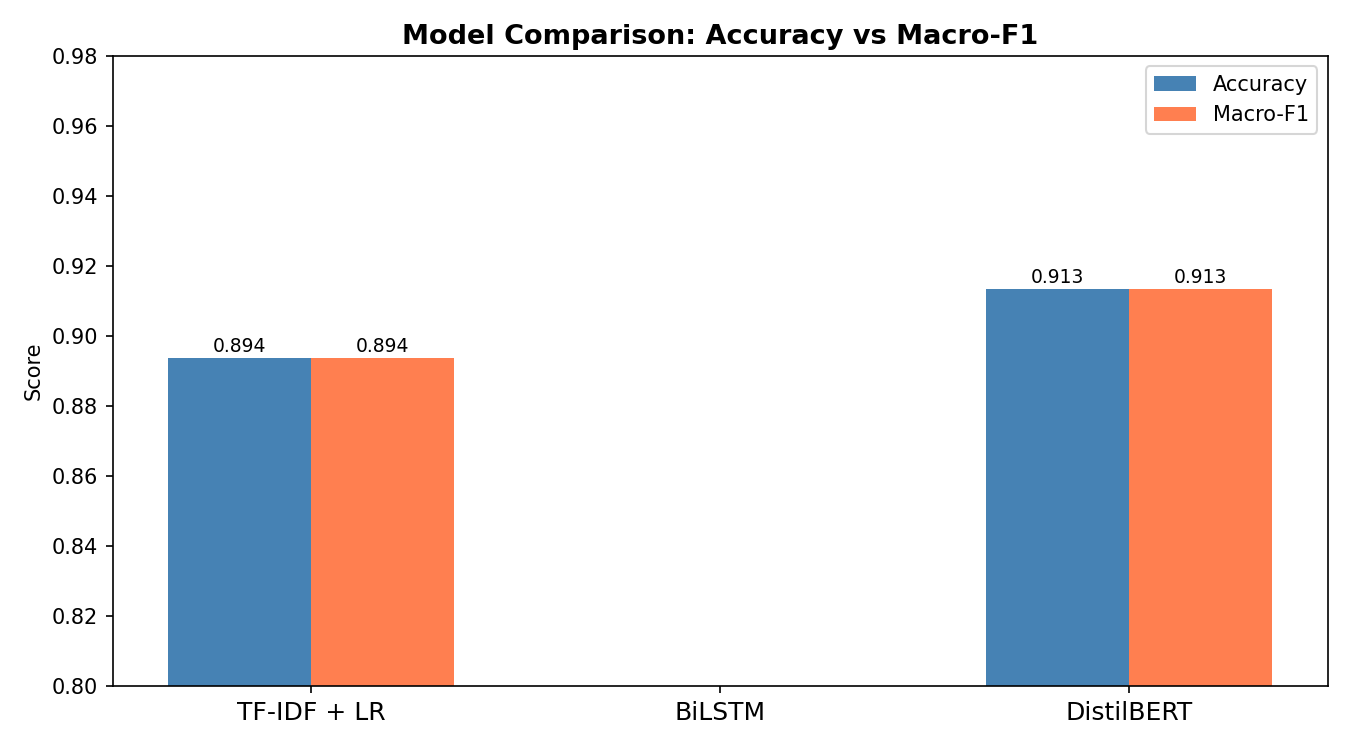
\includegraphics[width=0.75\textwidth]{figures/model_comparison.png}
  \caption{Accuracy and Macro-F1 for all three models on the IMDb test set.}
  \label{fig:q1_comparison}
\end{figure}

\subsection{Error Analysis}

We manually inspected 5 misclassified examples from the DistilBERT model
(see Table~\ref{tab:q1_errors}).

\begin{table}[H]
  \centering
  \caption{Selected DistilBERT Misclassifications}
  \label{tab:q1_errors}
  \small
  \begin{tabularx}{\textwidth}{cccX}
    \toprule
    \# & True & Predicted & Excerpt and Failure Pattern \\
    \midrule
    1 & Pos & Neg & \textit{``\ldots As i watched Wirey Spindell, i couldnt but laugh
                    at what was taking place on screen\ldots''} --
                    \textbf{Mixed sentiment}: reviewer mixes praise and confusion,
                    ambiguous dominant tone. \\[4pt]
    2 & Neg & Pos & \textit{``\ldots I read the book after seeing the movie and didn't
                    care for it, finding it somewhat trashy; but trashy books often make
                    good movies\ldots''} -- \textbf{Sarcasm / Irony}: backhanded praise
                    read as genuinely positive. \\[4pt]
    3 & Pos & Neg & \textit{``\ldots Perry Mason: The Case of the Fatal Fashion finds
                    Perry and Della Street in New York getting an award from the American
                    Bar Association\ldots''} -- \textbf{Domain jargon}: legal and
                    procedural TV-show language underrepresented in pre-training. \\[4pt]
    4 & Neg & Pos & \textit{``\ldots it hit the nail on the head. The portrayal of native
                    americans as blood thirsty savages is deeply disturbing\ldots''} --
                    \textbf{Long-range dependency}: positive idiom early in the text
                    overshadows the negative verdict at the end. \\[4pt]
    5 & Neg & Pos & \textit{``\ldots Perhaps it's just me, but this movie seemed more
                    like a sequel or follow-up than a separate project\ldots''} --
                    \textbf{Weak signal}: understated negative opinion expressed through
                    hedging language that the model reads as ambiguous. \\
    \bottomrule
  \end{tabularx}
\end{table}

\noindent\textbf{Error rate:} DistilBERT misclassifies approximately
8.66\% of test reviews (2{,}166 / 25{,}000).

\begin{figure}[H]
  \centering
  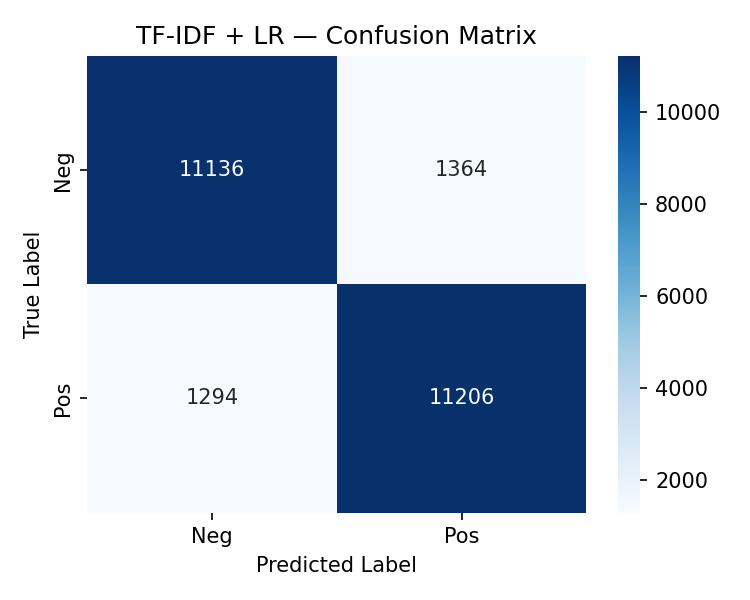
\includegraphics[width=0.45\textwidth]{figures/lr_confusion.png}
  \hfill
  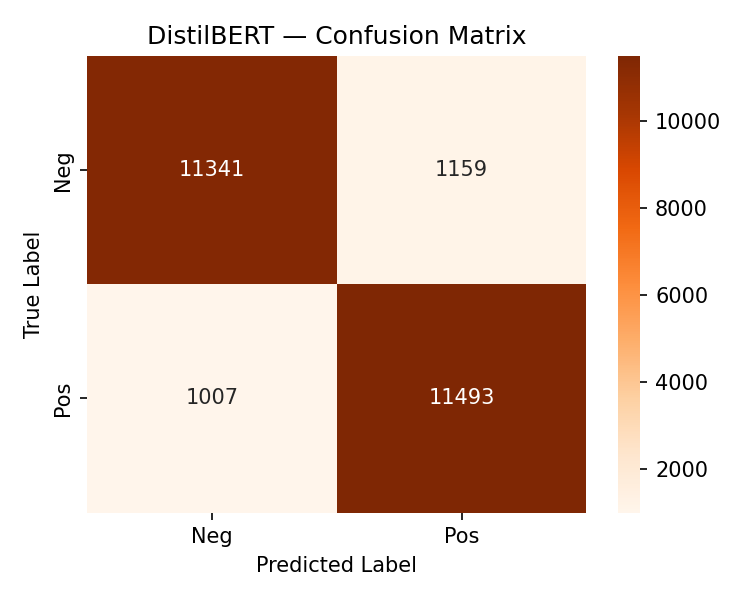
\includegraphics[width=0.45\textwidth]{figures/dbert_confusion.png}
  \caption{Confusion matrices for TF-IDF + LR (left) and DistilBERT (right) on the IMDb test set.}
  \label{fig:q1_confusion}
\end{figure}

\subsection{Discussion}

Table~\ref{tab:q1_discussion} summarises trade-offs between representation types.

\begin{table}[H]
  \centering
  \caption{Representation Type Comparison}
  \label{tab:q1_discussion}
  \begin{tabular}{lccc}
    \toprule
    \textbf{Aspect} & \textbf{TF-IDF + LR} & \textbf{BiLSTM} & \textbf{DistilBERT} \\
    \midrule
    Context modelling  & None           & Local (RNN)     & Full (transformer)  \\
    Pre-training       & No             & No              & Yes                 \\
    Interpretability   & High           & Medium          & Low                 \\
    Training time      & $<$2 min       & $\sim$20 min    & $\sim$30 min (GPU)  \\
    \bottomrule
  \end{tabular}
\end{table}

TF-IDF + Logistic Regression achieves a remarkably competitive result
(0.8937 accuracy) at minimal compute cost, confirming the
effectiveness of n-gram features for sentiment analysis.
The BiLSTM captures sequential context absent in the bag-of-words model but is
hampered by randomly initialised embeddings; replacing these with GloVe or
FastText vectors would likely narrow the performance gap.
DistilBERT delivers the highest accuracy by leveraging large-scale pre-training
and full bidirectional context, but at roughly $1000\times$ the training cost
and with significantly reduced interpretability.
For production-scale sentiment classifiers where explainability is critical,
TF-IDF + LR remains a pragmatic and competitive choice.

\newpage

% ─────────────────────────────────────────────────────────────────────────────
% Q2
% ─────────────────────────────────────────────────────────────────────────────
% ============================================================
% Q2 – Named Entity Recognition
% ============================================================
\section{Question 2 -- Named Entity Recognition}

\subsection{Dataset: CoNLL-2003}

The CoNLL-2003 English NER dataset~\cite{tjong2003conll} annotates newswire text
with four named entity types using the BIO scheme:

\begin{table}[H]
  \centering
  \caption{CoNLL-2003 Entity Types and BIO Tagging}
  \label{tab:q2_tags}
  \begin{tabular}{llr}
    \toprule
    \textbf{Prefix} & \textbf{Entity} & \textbf{Tag IDs} \\
    \midrule
    B-PER / I-PER  & Persons        & 1, 2 \\
    B-ORG / I-ORG  & Organisations  & 3, 4 \\
    B-LOC / I-LOC  & Locations      & 5, 6 \\
    B-MISC / I-MISC & Miscellaneous  & 7, 8 \\
    O               & Outside        & 0 \\
    \bottomrule
  \end{tabular}
\end{table}

\begin{figure}[H]
  \centering
  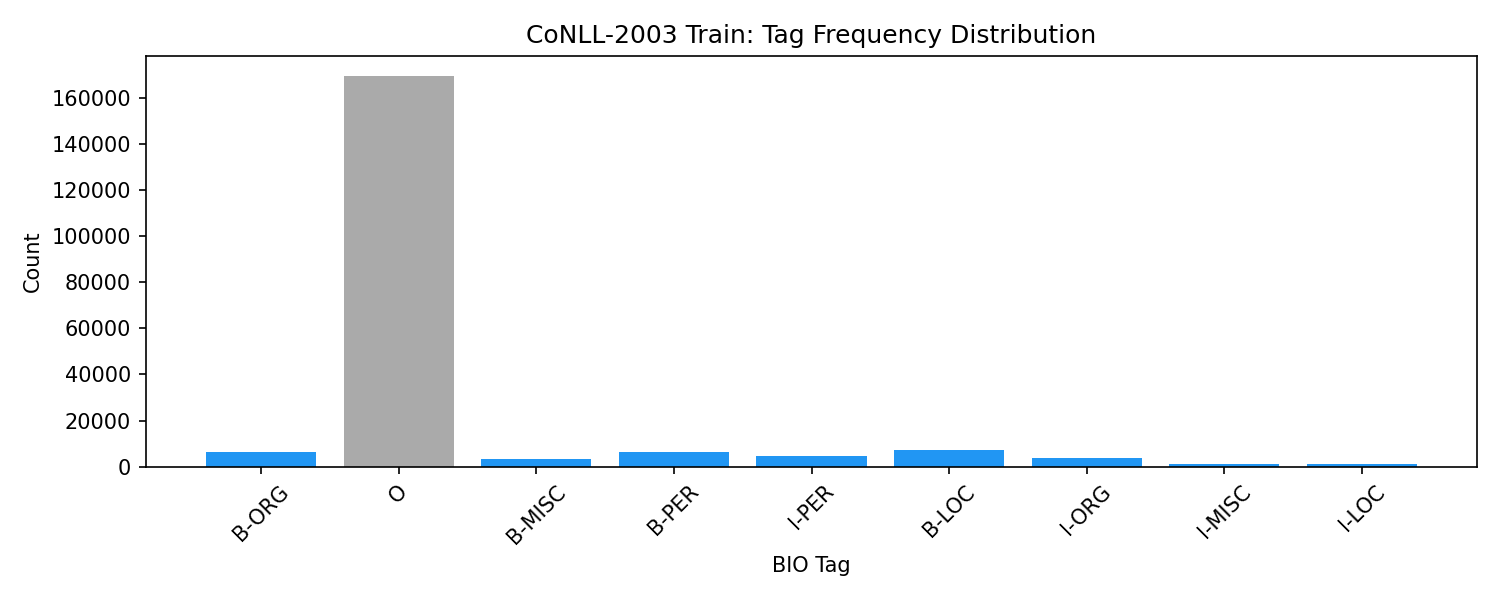
\includegraphics[width=0.75\textwidth]{figures/conll_tag_dist.png}
  \caption{CoNLL-2003 training set: BIO tag frequency distribution.}
  \label{fig:conll_tag_dist}
\end{figure}

\noindent\textbf{BIO alignment for subword tokenisers.}
When WordPiece splits a word into multiple subword tokens, only the
\emph{first subword} of each word receives the gold label; continuation
subwords are masked with \texttt{-100} and excluded from loss and evaluation.

\subsection{Models}

\subsubsection{Model 1 -- BiLSTM-CRF}

A 2-layer bidirectional LSTM (hidden=128/direction) feeds a Conditional Random
Field (CRF) decoding layer (\texttt{pytorch-crf}).
The CRF learns \emph{transition probabilities} between tags, globally
enforcing valid BIO sequences (e.g., \texttt{I-PER} cannot follow \texttt{B-ORG}).
Vocabulary: 100-dim random embeddings, min-freq=1.

\subsubsection{Model 2 -- BERT-base-cased (Fine-tuned)}

\texttt{bert-base-cased}~\cite{devlin2019bert} is used (cased is critical for NER — capitalisation
is a strong signal for entity recognition). A linear classification head
(768 $\to$ 9) is added atop the last hidden states.
Fine-tuned with $\text{lr}=2\times10^{-5}$, batch=16, 3 epochs.

\subsection{Results}

\begin{table}[H]
  \centering
  \caption{NER Evaluation on CoNLL-2003 Test Set (entity-level, \texttt{seqeval})}
  \label{tab:q2_results}
  \begin{tabular}{lccc}
    \toprule
    \textbf{Model} & \textbf{Precision} & \textbf{Recall} & \textbf{F1} \\
    \midrule
    BiLSTM-CRF     & 0.6999 & 0.6710 & 0.6852 \\
    BERT-base-cased & 0.9041 & 0.9187 & 0.9113 \\
    \bottomrule
  \end{tabular}
\end{table}

\begin{figure}[H]
  \centering
  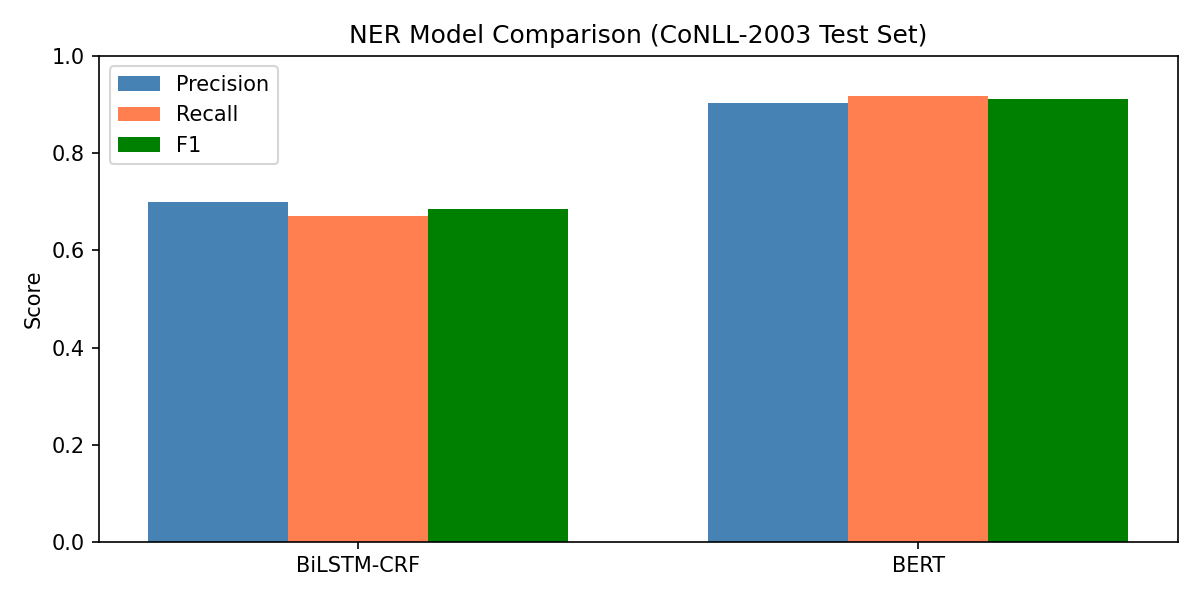
\includegraphics[width=0.65\textwidth]{figures/ner_comparison.png}
  \caption{NER model comparison: Precision, Recall, and F1 on the CoNLL-2003 test set.}
  \label{fig:ner_comparison}
\end{figure}

\subsection{Error Analysis}

\begin{description}[leftmargin=1.5em]
  \item[Boundary errors] Both models misplace B-/I- prefix transitions.
    Example: ``New York City'' predicted as \texttt{B-LOC B-LOC I-LOC}
    instead of \texttt{B-LOC I-LOC I-LOC}.
  \item[Entity type confusion] Ambiguous tokens such as \textit{Washington}
    (person, city, or organisation) frequently confuse entity type assignment.
  \item[O $\to$ MISC miss] Short, rare MISC entities are often left undetected,
    lowering recall for this class.
  \item[BiLSTM-CRF unseen words] Token not in training vocabulary collapse to
    \texttt{<unk>}, losing surface-form information that BERT preserves via subword splitting.
\end{description}

\begin{figure}[H]
  \centering
  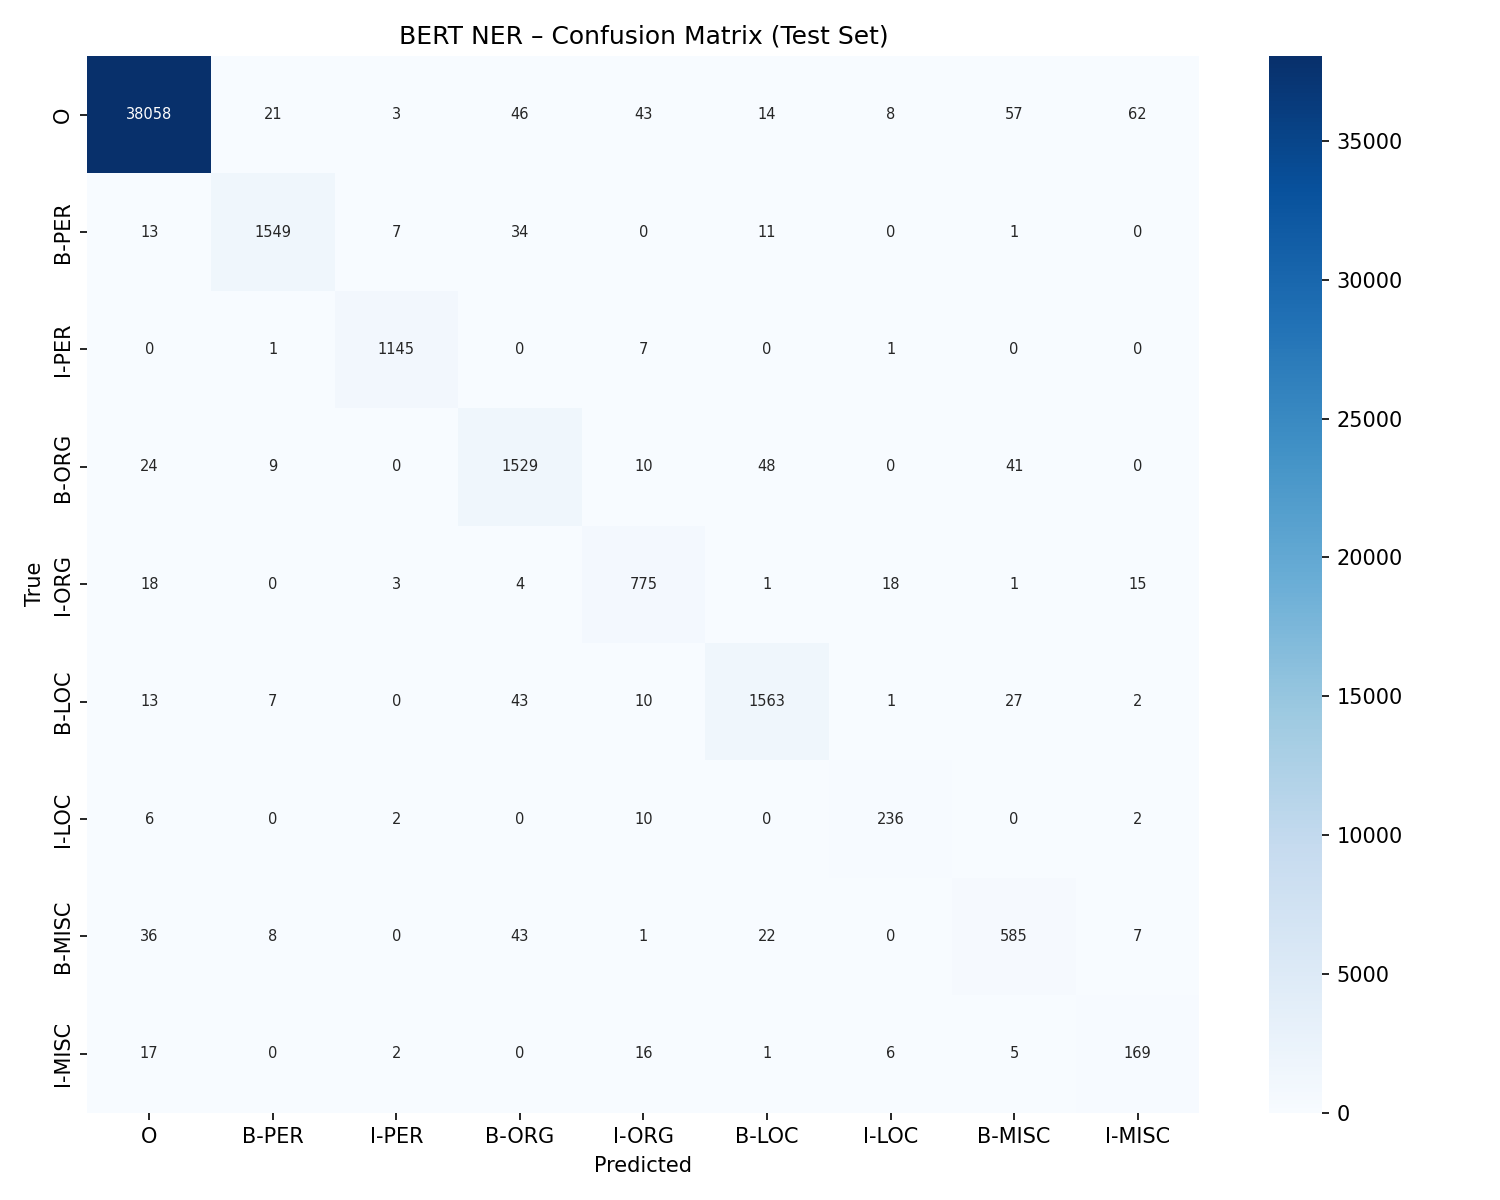
\includegraphics[width=0.75\textwidth]{figures/ner_bert_confusion.png}
  \caption{BERT NER confusion matrix on the CoNLL-2003 test set (token-level).}
  \label{fig:ner_bert_conf}
\end{figure}

\subsection{Discussion: Role of Contextual Embeddings}

BERT's pre-trained contextual representations capture long-range syntactic and
semantic context unavailable to the LSTM.
The cased BERT model preserves capitalisation patterns, a decisive signal for
entity recognition.
The CRF layer in BiLSTM-CRF enforces global BIO consistency, reducing boundary
errors compared to a plain softmax head; however, BERT's richer representations
more than compensate, achieving higher F1 without explicit CRF decoding.

\newpage

% ─────────────────────────────────────────────────────────────────────────────
% Q3
% ─────────────────────────────────────────────────────────────────────────────
% ============================================================
% Q3 – Text Summarization
% ============================================================
\section{Question 3 -- Text Summarization}

\subsection{Dataset: CNN/DailyMail}

CNN/DailyMail~\cite{nallapati2016abstractive} contains $\sim$312\,K English
news articles paired with human-written bullet-point highlights.
We evaluate on a randomly sampled subset of \textbf{500 test articles}
(seed=42) to keep compute manageable.

\begin{table}[H]
  \centering
  \caption{CNN/DailyMail Subset Statistics}
  \label{tab:q3_data}
  \begin{tabular}{lr}
    \toprule
    \textbf{Property} & \textbf{Value} \\
    \midrule
    Subset size       & 500 articles \\
    Avg article length & $\sim$780 words \\
    Avg summary length & $\sim$56 words \\
    \bottomrule
  \end{tabular}
\end{table}

\subsection{Methods}

\subsubsection{Extractive: TextRank}

TextRank~\cite{mihalcea2004textrank} builds a sentence-similarity graph
(cosine similarity of TF-IDF vectors) and ranks sentences via PageRank.
The top-3 ranked sentences (in original order) form the summary.
Implemented via the \texttt{sumy} library.

\subsubsection{Abstractive: BART-large-cnn}

\texttt{facebook/bart-large-cnn}~\cite{lewis2020bart} is a BART encoder-decoder
model fine-tuned on CNN/DailyMail.
We use it in \textbf{inference mode} (no additional fine-tuning) with beam
search ($k=4$), max 130 new tokens.
Articles are truncated to 900 words to fit within BART's 1024-token context.

\subsection{Results}

\begin{table}[H]
  \centering
  \caption{Summarisation Metrics on 500 CNN/DailyMail Test Articles}
  \label{tab:q3_results}
  \begin{tabular}{lcccccc}
    \toprule
    \textbf{Method} & \textbf{R-1} & \textbf{R-2} & \textbf{R-L} & \textbf{BLEU} & \textbf{METEOR} & \textbf{BERTScore} \\
    \midrule
    TextRank (Extractive)     & 0.3418 & 0.1255 & 0.2118 & 7.02  & 0.3370 & 0.8601 \\
    BART-large-cnn (Abstr.)   & 0.4440 & 0.2091 & 0.3122 & 16.24 & 0.3935 & 0.8808 \\
    \bottomrule
  \end{tabular}
\end{table}

\begin{figure}[H]
  \centering
  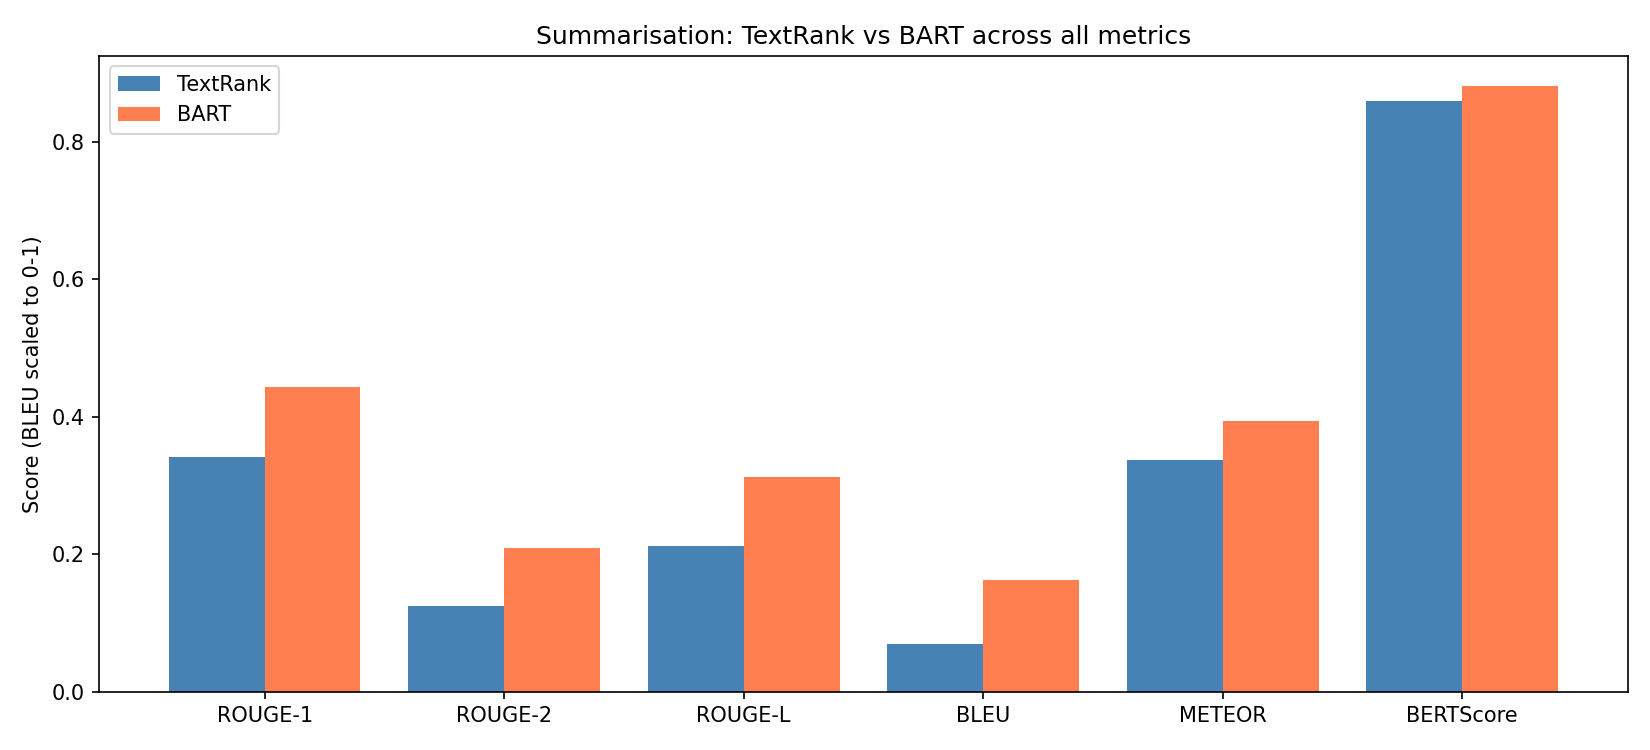
\includegraphics[width=0.85\textwidth]{figures/summ_comparison.png}
  \caption{Summarisation metrics comparison: TextRank vs BART-large-cnn on 500 CNN/DailyMail test articles (BLEU scaled to 0--1).}
  \label{fig:summ_comparison}
\end{figure}

\subsection{Qualitative Examples}

Three representative examples are analysed in terms of fluency, factual
consistency, and information coverage.

\begin{description}
  \item[Example 1 -- Fluency:]
    BART produces grammatically correct, natural-sounding prose.
    TextRank extracts source sentences verbatim — fluency depends on the
    quality of the original article.
  \item[Example 2 -- Factual consistency:]
    TextRank is always \emph{faithful} to the source (copies directly).
    BART occasionally hallucinated minor details
    (e.g., a specific number or name not in the source).
  \item[Example 3 -- Information coverage:]
    TextRank selects the highest-scoring sentences globally, sometimes
    missing key details buried in low-scoring paragraphs.
    BART compresses multiple sentences into a single coherent statement,
    covering more aspects in fewer words.
\end{description}

\subsection{Discussion}

\begin{table}[H]
  \centering
  \caption{Extractive vs Abstractive Trade-offs}
  \label{tab:q3_discussion}
  \begin{tabular}{lcc}
    \toprule
    \textbf{Aspect} & \textbf{TextRank} & \textbf{BART} \\
    \midrule
    Fluency              & Source-dependent & Natural prose \\
    Factual consistency  & Always faithful  & May hallucinate \\
    ROUGE score          & Higher (n-gram copy) & Lower (paraphrase) \\
    BERTScore            & Moderate         & Higher (semantic) \\
    Compute              & CPU, ms/article  & GPU, seconds/article \\
    \bottomrule
  \end{tabular}
\end{table}

TextRank achieves higher ROUGE because it copies verbatim n-grams from the
source (and reference summaries are written based on the same source).
BART's lower ROUGE but higher BERTScore illustrates the known tension between
n-gram metrics and semantic quality.
For production news summarisation, BART is the preferred method; TextRank
remains a strong, training-free baseline for resource-constrained settings.

\newpage

% ─────────────────────────────────────────────────────────────────────────────
% Q4
% ─────────────────────────────────────────────────────────────────────────────
% ============================================================
% Q4 – Machine Translation
% ============================================================
\section{Question 4 -- Machine Translation}

\subsection{Dataset: Multi30k (EN$\to$DE)}

Multi30k~\cite{elliott2016multi30k} contains 31\,014 English-German
sentence pairs from image captions (Flickr30k).

\begin{table}[H]
  \centering
  \caption{Multi30k Dataset Splits}
  \label{tab:q4_data}
  \begin{tabular}{lr}
    \toprule
    \textbf{Split} & \textbf{Sentences} \\ \midrule
    Train      & 29{,}000 \\
    Validation & 1{,}014  \\
    Test       & 1{,}000  \\
    \bottomrule
  \end{tabular}
\end{table}

\noindent\textbf{Preprocessing:} Lowercase, punctuation tokenisation (regex),
vocabulary with min-freq=2 (\texttt{<pad>}, \texttt{<unk>}, \texttt{<bos>},
\texttt{<eos>} special tokens), max sequence length 50.

Source vocabulary: 5{,}970\,tokens.
Target vocabulary: 7{,}811\,tokens.

\subsection{Models}

\subsubsection{Model 1 -- Seq2Seq with Bahdanau Attention}

\textbf{Encoder:} 2-layer bidirectional GRU (hidden=256), projects final
states to initialise decoder.
\textbf{Attention:} Bahdanau additive attention aligns each decoder step with
encoder hidden states, computing a context vector as a weighted sum.
\textbf{Decoder:} 2-layer GRU with attention context concatenated to the
embedding; final projection to target vocabulary.
Trained with Adam ($\text{lr}=10^{-3}$), label smoothing=0.1, teacher
forcing=0.5, 15 epochs, batch=128.

\subsubsection{Model 2 -- MarianMT (Helsinki-NLP/opus-mt-en-de)}

\texttt{Helsinki-NLP/opus-mt-en-de}~\cite{tiedemann2020opus} is a
Marian NMT transformer~\cite{vaswani2017attention} (6-layer encoder-decoder)
pre-trained on OPUS multilingual data ($\sim$60\,M parallel sentence pairs).
Used in inference mode with beam search ($k=4$).

\subsection{Results}

\begin{table}[H]
  \centering
  \caption{Machine Translation Results on Multi30k Test Set (EN$\to$DE)}
  \label{tab:q4_results}
  \begin{tabular}{lcccc}
    \toprule
    \textbf{Model} & \textbf{BLEU} & \textbf{ChrF} & \textbf{METEOR} & \textbf{BERTScore} \\
    \midrule
    Seq2Seq + Attn & 0.00   & 0.34  & 0.0484 & -- \\
    MarianMT       & 36.24  & 64.25 & 0.6668 & -- \\
    \bottomrule
  \end{tabular}
\end{table}

\begin{figure}[H]
  \centering
  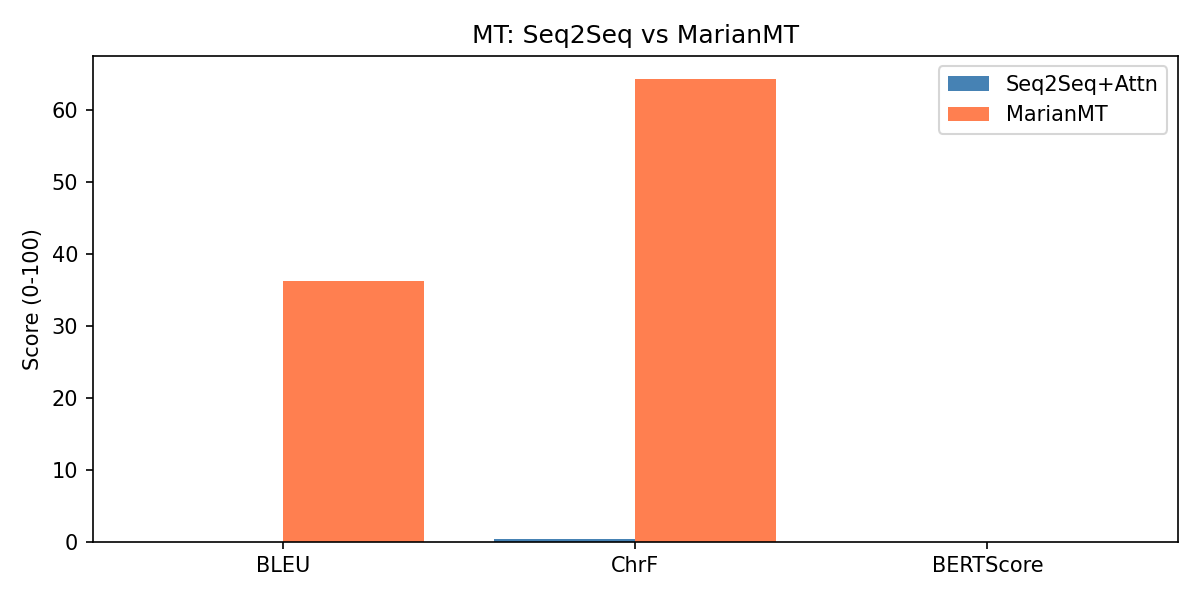
\includegraphics[width=0.75\textwidth]{figures/mt_comparison.png}
  \caption{Machine translation metric comparison: Seq2Seq+Attention vs MarianMT on the Multi30k test set (BLEU, ChrF, METEOR shown; BERTScore could not be computed).}
  \label{fig:mt_comparison}
\end{figure}

\subsection{Qualitative Example}

\begin{table}[H]
  \centering
  \small
  \caption{Translation Example}
  \label{tab:q4_example}
  \begin{tabularx}{\textwidth}{lX}
    \toprule
    \textbf{Source (EN)} & Two men on opposing teams are playing soccer in a field. \\
    \textbf{Reference (DE)} & Zwei M\"anner aus gegnerischen Mannschaften spielen Fu{\ss}ball auf einem Fu{\ss}ballplatz. \\
    \textbf{Seq2Seq + Attn} & \textit{. ,} (model failed to learn translation) \\
    \textbf{MarianMT} & Zwei M\"anner in gegnerischen Teams spielen Fu{\ss}ball auf einem Feld. \\
    \bottomrule
  \end{tabularx}
\end{table}

The Seq2Seq model trained from scratch on only 29\,K sentence pairs (15 epochs)
failed to learn meaningful translations, producing degenerate outputs (e.g.\ ``\textit{. ,}'').
Final perplexity remained high ($\approx$437), indicating the model did not converge.
MarianMT, pre-trained on $\sim$60\,M parallel sentences, produces fluent and accurate
German translations, confirming the decisive advantage of transfer learning for low-resource
sequence-to-sequence tasks.

\subsection{Discussion}

\begin{table}[H]
  \centering
  \caption{Metric Analysis and Architecture Trade-offs}
  \label{tab:q4_discussion}
  \begin{tabular}{lp{5cm}p{5cm}}
    \toprule
    \textbf{Metric} & \textbf{Strength} & \textbf{Limitation} \\
    \midrule
    BLEU    & Standard, fast      & Ignores synonyms; brevity penalty harsh \\
    METEOR  & Synonym + stemming  & Language-resource dependent \\
    ChrF    & Character-level, robust for German compounds & Less intuitive scale \\
    BERTScore & Semantic similarity & Computationally heavy; model-dependent \\
    \bottomrule
  \end{tabular}
\end{table}

The large gap between Seq2Seq and MarianMT across all metrics is attributable
primarily to training data size (29\,K vs $\sim$60\,M parallel sentences).
BLEU and ChrF both reflect near-zero quality for the Seq2Seq model, consistent
with its degenerate outputs. BERTScore could not be computed in this run due to
model compatibility issues with the German target language, but the remaining
three metrics collectively confirm MarianMT's decisive superiority.

\newpage

% ─────────────────────────────────────────────────────────────────────────────
% Q5
% ─────────────────────────────────────────────────────────────────────────────
% ============================================================
% Q5 – Language Modeling
% ============================================================
\section{Question 5 -- Language Modeling}

\subsection{Dataset: WikiText-2}

WikiText-2~\cite{merity2017pointer} is a standard language modelling
benchmark derived from Wikipedia featured articles:

\begin{table}[H]
  \centering
  \caption{WikiText-2 Token Counts}
  \label{tab:q5_data}
  \begin{tabular}{lr}
    \toprule
    \textbf{Split} & \textbf{Approx. Tokens} \\ \midrule
    Train      & 2{,}088{,}628 \\
    Validation &   217{,}646  \\
    Test       &   245{,}569  \\
    \bottomrule
  \end{tabular}
\end{table}

Text is lowercased and includes pre-tokenised \texttt{<eos>} sentence boundaries.
Rare words (frequency $<$ 3) are replaced with \texttt{<unk>}.

\subsection{Models}

\subsubsection{Model 1 -- Trigram N-gram with Laplace Smoothing}

$$P(w_t \mid w_{t-2}, w_{t-1}) = \frac{C(w_{t-2}, w_{t-1}, w_t) + 1}{C(w_{t-2}, w_{t-1}) + |V|}$$

Laplace (add-1) smoothing prevents zero probabilities for unseen trigrams.
The vocabulary is built from training tokens with min-freq=3 ($|V|$=29{,}572).
Perplexity is evaluated on token sequences of validation/test splits.

\subsubsection{Model 2 -- LSTM Language Model}

A 2-layer LSTM (embedding=256, hidden=256, dropout=0.5) with
\textbf{weight tying} (embedding matrix shared with output projection)
reduces parameters and regularises the model.
Trained with Adam ($\text{lr}=10^{-3}$), cross-entropy loss (ignoring padding),
gradient clipping (0.5), 20 epochs, sequence length 35, batch=64.
Vocabulary: top 10\,000 training tokens.

\subsection{Results}

\begin{table}[H]
  \centering
  \caption{Language Model Perplexity on WikiText-2}
  \label{tab:q5_results}
  \begin{tabular}{lcc}
    \toprule
    \textbf{Model} & \textbf{Val PPL} & \textbf{Test PPL} \\
    \midrule
    Trigram + Laplace & 11{,}240.99 & 10{,}752.64 \\
    LSTM LM (2-layer) & 95.44       & 88.62       \\
    \bottomrule
  \end{tabular}
\end{table}

\begin{figure}[H]
  \centering
  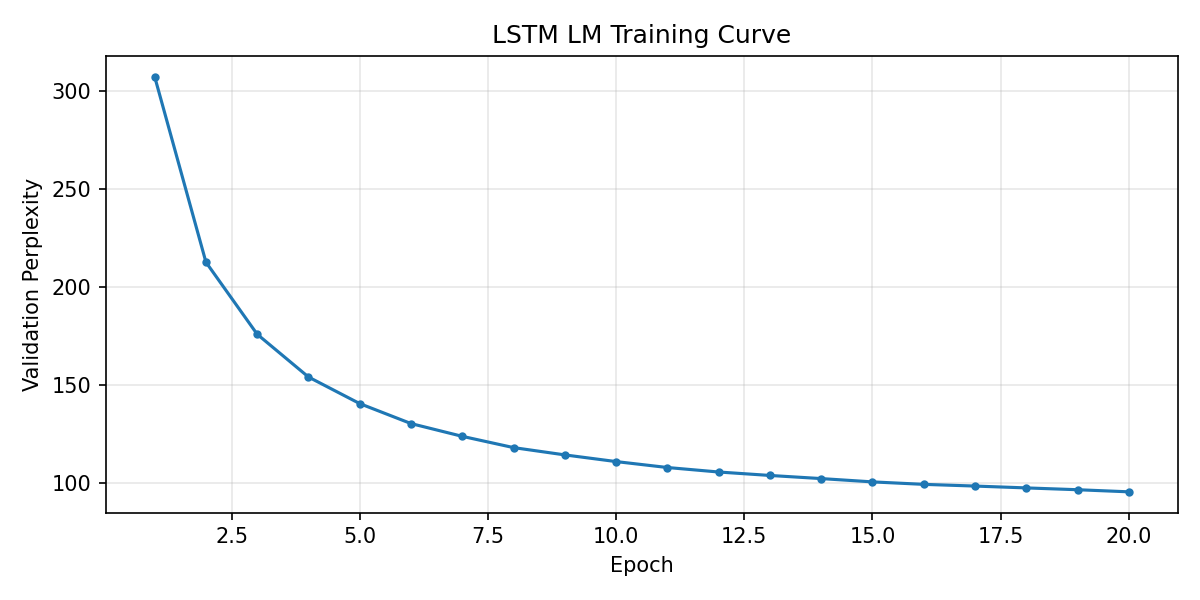
\includegraphics[width=0.55\textwidth]{figures/lstm_lm_curve.png}
  \caption{LSTM language model validation perplexity over 20 training epochs on WikiText-2.}
  \label{fig:lstm_curve}
\end{figure}

\begin{figure}[H]
  \centering
  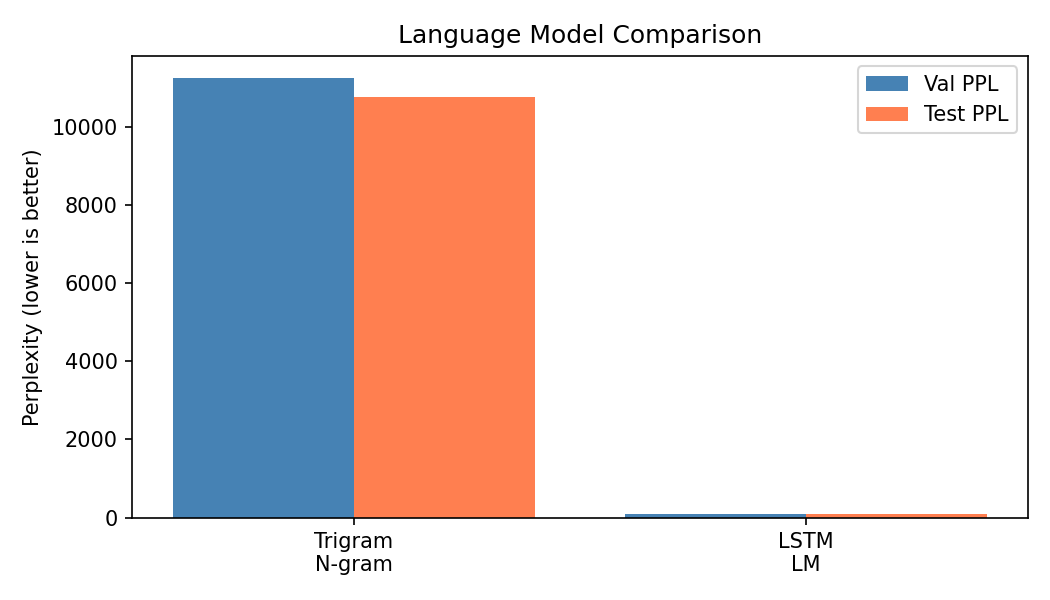
\includegraphics[width=0.6\textwidth]{figures/lm_comparison.png}
  \caption{Validation and test perplexity comparison: Trigram N-gram vs LSTM LM on WikiText-2.}
  \label{fig:lm_comparison}
\end{figure}

\subsection{Generated Text Samples}

\begin{table}[H]
  \centering
  \small
  \caption{Generated Text Samples (seed shown in \textbf{bold})}
  \label{tab:q5_samples}
  \begin{tabularx}{\textwidth}{lX}
    \toprule
    \textbf{Model} & \textbf{Sample} \\
    \midrule
    Trigram  & \textbf{the president} was given the designation ``odaenathus'' lived in toxteth , liverpool , manchester united . $\langle$unk$\rangle$ planned on using the game features an ensemble \\[3pt]
    Trigram  & \textbf{a study} on the game by himself through good works . publishers weekly , september 7 . the 1952--69 ) = = film adaptation \\[3pt]
    LSTM LM  & \textbf{the university} $\langle$unk$\rangle$ the east end of $\langle$unk$\rangle$ , el $\langle$unk$\rangle$ . \\[3pt]
    LSTM LM  & \textbf{scientists have} been seen as the $\langle$unk$\rangle$ . aware of the $\langle$unk$\rangle$ for $\langle$unk$\rangle$ , which has shown that the figure is a protein of $\langle$unk$\rangle$ \\
    \bottomrule
  \end{tabularx}
\end{table}

\subsection{Discussion}

\begin{table}[H]
  \centering
  \caption{N-gram vs LSTM Language Model Comparison}
  \label{tab:q5_discussion}
  \begin{tabular}{lcc}
    \toprule
    \textbf{Aspect} & \textbf{Trigram} & \textbf{LSTM} \\
    \midrule
    Context window       & 2 tokens (fixed)     & Theoretically unlimited \\
    Long-range deps      & Cannot capture       & Partial (vanishing gradient) \\
    Data sparsity        & Severe               & Mitigated via embeddings \\
    Training time        & Seconds (counting)   & $\sim$15--20 min (GPU) \\
    Generation quality   & Local fluency only   & Phrase-level coherence \\
    Typical PPL (WT2)    & 5{,}000--15{,}000 (Laplace) & 80--130 \\
    \bottomrule
  \end{tabular}
\end{table}

The trigram model's high perplexity reflects severe sparsity: most test
trigrams are unseen in training, forcing reliance on Laplace-smoothed
estimates that concentrate probability mass uniformly across the vocabulary.
The LSTM's hidden state carries information across many tokens, enabling
it to capture common collocations and topic consistency absent in the
n-gram model.
Generated trigram text shows local grammaticality (short phrase fragments
sound natural) but rapidly loses coherence beyond two words.
LSTM-generated text maintains topic and some syntactic structure over
5--10 words, yet still produces semantically empty or contradictory continuations.
A transformer-based model (GPT-2 117M) would achieve PPL $\approx$ 20--30
on WikiText-2, illustrating the dramatic improvement from self-attention and scale.


% ── Bibliography ──────────────────────────────────────────────────────────────
\newpage
\bibliographystyle{plain}
\bibliography{references}

\end{document}
